% \section{CUIT}
% Annahmen: es gibt ein Fenster mit \code{Title="Login Window"}. In diesem Fenster gibt es zwei \code{Textbox}en mit LoginName und Password (Attribut \code{Name=}), und einen \code{Button} der sich LoginButton nennt. Stimmt das Login, so öffnet sich ein Fenster mit dem Titel \code{"Welcome Window"}, welches ein \code{Label} mit dem Namen NameLabel besitzt.

% Wir wollen nun den Usernamen und das Passwort abfüllen, OK klicken, und sehen ob das korrekte Fenster aufgeht.

% \begin{lstlisting}
% [TestClass]
% public class LoginWindowUiTest
% {
%   // Das Folgende kann immer gleich implementiert werden
%   // the directory in which the test is running
%   public string BaseDir => Path.GetDirectoryName(Assembly.GetExecutingAssembly().Location);
%   // system under test (wpf app to be tested)
%   public string SutPath => Path.Combine(BaseDir, $"ch.hsr.wpf.03.login.exe");
  
%   [TestMethod]
%   public void TestMethod1()
%   {
%   var app = Application.Launch(SutPath);
%   var window = app.GetWindow("Login Window", InitializeOption.NoCache);
%   var name = window.Get<TextBox>("LoginName");
%   var pw = window.Get<TextBox>("Password");
%   name.Text = "j.bond";
%   pw.Text = "topsecret";
%   var button = window.Get<Button>("LoginButton");
%   button.Click();
%   var win = app.GetWindow("Welcome Window", InitializeOption.NoCache);
%   var label = win.Get<Label>("NameLabel");
%   Assert.AreEqual("j.bond", label.Text);
%   win.Close();
%   app.Close();
%   }
  
% }
% \end{lstlisting}



\section{MVVM}
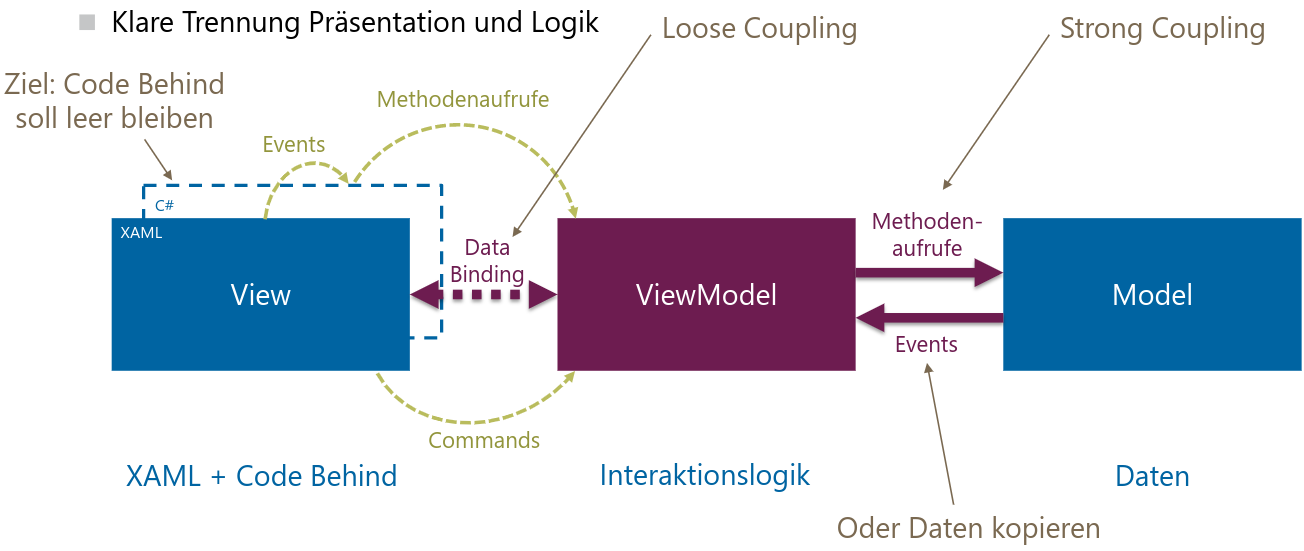
\includegraphics[scale=0.27, angle=90]{img/mvvm_uebersicht.png}

\paragraph{Model} 
\begin{itemize}
    \item Eigentliche Daten
    \item Domain Objekte haben kein Verhalten
    \item Nicht zuständig für: Formatierung, Laden, Speichern
\end{itemize}

\paragraph{ViewModel} 
\begin{itemize}
    \item View-spezifische Objekte, welche die Domain Objekte um Daten, Berechnungen für die View anreichern
    \item ''Butler'' für eine View, präsentiert alles auf dem Silbertablett
    \item Zuständig für die Darstellung und Formatierung der Daten im Hinblick auf die Darstellung der View
    \item Grundlage für stressfreies DataBinding
\end{itemize}
\textbf{Bilanz}
\begin{itemize}
    \item Modelklassen bleiben einfache POCOs
    \item ViewModels teilen via PropertyChanged-Event mit, wenn sich etwas ändert
    \item ViewModels sind somit für DataBindingvorbereitet 
    \item Fleissarbeit (Kopieren von Properties) übernimmt Library (z.B. AutoMapper) 
    \item Aktionen können via Commands ausgelöst werden 
    \item ViewModels sind testbar, da keine direkte Verdrahtung mit UI-Code
\end{itemize}

\paragraph{Zusammenarbeit Model $\Leftrightarrow$ ViewModel}
Ganzes Model als Property kapseln (nützt nur etwas, wenn sich ganzes Model ändert)
\begin{lstlisting}[language=sharpc]
public class GadgetVm:BindableBase { 
  private Gadget _gadget;
  public Gadget Gadget { 
    get { return _gadget; }
    set { SetProperty(ref _gadget, value, nameof(Gadget));
    }
}
//eventuell noch anderer Code
} 
\end{lstlisting}

Für jede im UI benötigte Property eine gleichnamige VM-Property implementieren (Fleissarbeit $\Rightarrow$ automapper verwenden)
\begin{lstlisting}[language=sharpc]
public class GadgetVm:BindableBase 
{ 
  private string _inventoryNumber; 
  public string InventoryNumber 
  { 
    get { return _inventoryNumber; } 
    set { SetProperty(ref _inventoryNumber, value, nameof(InventoryNumber)); } 
  } 
  //eventuell noch anderer Code 
}
\end{lstlisting}

\paragraph{View} 
\begin{itemize}
    \item XAML + Code Behind (wenig)
    \item Zustände via Data Binding zwischenspeichern
    \item Designs: Styles mit Control Templates
    \item Layouts: UserControl
    \item Möglichst so schreiben, dass viele Teile wiederverwendet werden können
    \item Möglichst wenig (am besten kein) Zugriff auf die UI Controls aus dem Code Behind (Thema Kopplung)
    \item Zustände im DataBinding speichern
    \item 
\end{itemize}

%\paragraph{Anmerkung} Auf Interfaces Referenzieren die eine andere Komponente implementiert ist ok.




\subsection{Commands}
\begin{description}
    \item[\code{ICommand}] im ViewModel implementieren und dann via DataBinding auslösen
    \item[Vorteil:] View weiss nichts vom ViewModel und löst nur Aktionen (Commands) aus
    \item[Command] führt die Aktion (z.B speichern) aus
    \item[Command Source] ist das UI-Controls (z.B Button), welcher auf ein Event (z.B Click) reagiert und dann die Aktion (Command) auslöst.
    \item[Command Binding] wird definiert auf dem UI-Control (z.B Button), so dass dieses UI-Control das Kommando beim Event (z.B Klicken) auslöst
\end{description}

\paragraph{Nutzung}
Command werden beim DataBinding wie gewohnt angegeben:
\begin{lstlisting}[language=xml]
<Button Content="Save" Command="{Binding SaveCommand}" /> 
\end{lstlisting}
Falls zusätzliche Parameter übermittelt werden sollen:
\begin{lstlisting}[language=xml]
<Button Content="Open" Command="{Binding OpenGadgetViewCommand}" CommandParameter="{Binding SelectedAuto}" /> 
\end{lstlisting}

\paragraph{Implementierung/Beispiel von Commands}

Eigene Command-Klasse, Instanz davon als Property im ViewModel.
\textbf{Nachteil:} Kein Zugriff auf private Member des ViewModels 
\begin{lstlisting}[language=sharpc]
public class SomeCommand : ICommand { 
  public bool CanExecute(object parameter) { // ... irgendwie true oder false zurückgeben }
  public void Execute(object parameter) { // ... irgendwas ausführen } 
  public event EventHandler CanExecuteChanged;
} 
\end{lstlisting}

\begin{lstlisting}[language=sharpc]
public class GadgetVm:BindableBase { 
  // streng getypt, oder auch nur ICommand:
  public SomeCommand MyCommand { get; set; }
  // public ICommand MyCommand { get; set; } 
  public GadgetVm() {
  MyCommand = new SomeCommand(); 
  } //weiterer Code }
\end{lstlisting}

Command als innere Klasse im ViewModel implementieren.
\textbf{Vorteil} Zugriff auf private Member des ViewModels

\begin{lstlisting}[language=sharpc]
public class GadgetVm:BindableBase // Start des ViewModels {
   ...
   public class SomeCommand : ICommand // Start des Commands { 
     public bool CanExecute(object parameter) { // ... irgendwie true oder false zurückgeben }
     public void Execute(object parameter) { // ... irgendwas ausführen // ... jetzt aber mit Zugriff auf private Members } public event EventHandler CanExecuteChanged;
     private GadgetVm ViewModel { get; set; } 
     // eine Instanz auf das ViewModel übergeben:
     public SomeCommand(GadgetVm vm) { ViewModel = vm; } 
   } // Ende des Kommandos ... 
} // Ende des ViewModels 
     
\end{lstlisting}

\subsection{RelayCommand}
''Command-Pattern'', das man selber implementieren muss, aber dann viel Zeit und Geld spart (Ziit und Geld han ich kei).

Nicht-generic RelayCommand
\begin{lstlisting}
public class RelayCommand : ICommand
{
    private readonly Action _execute;
    private readonly Func<bool> _canExecute;
    
    public RelayCommand(Action execute, Func<bool> 
        canExecute = null)
    {
        if (execute == null) throw new 
            ArgumentNullException("execute");
        
        _execute = execute;
        _canExecute = canExecute;
    }
    
    public bool CanExecute(object parameter) => 
        _canExecute?.Invoke() ?? True
    public void Execute(object parameter) => _execute();
    
    // Event an CommandManager delegieren (Benachrichtigung erfolgt
    // so immer dann wenn WPF denkt, dass sich etwas am Ausführungs- 
    // status geändert hat, z.B. bei Key- oder Mouse-Button-Klick)
    public event EventHandler CanExecuteChanged
    {
        add { CommandManager.RequerySuggested += value; }
        remove { CommandManager.RequerySuggested += value }
    }
}
\end{lstlisting}

Die Generic-Variante nutzt ein \mintinline{csharp}{Action<T>} als \mintinline{csharp}{_execute} und ein \mintinline{csharp}{Predicate<T>} als \mintinline{csharp}{_canExecute}

Verwendung:

\begin{lstlisting}
public class GadgetVm : BindableBase
{
    public ICommand SaveCommand { get; set; }
    
    public GadgetVm()
    {
        SaveCommand = new RelayCommand(
            () => this.Save(), // Methode des ViewModels
            () => this.CanSave // Property des ViewModels
        );
    }
    
    public CanSave => ; // some condition
    public void Save() {} // some method
}
\end{lstlisting}

\subsection{ViewModel vs View}
\begin{itemize}
    \item ViewModel kennt die View nicht
    \begin{itemize}
    \item Keine Referenz auf die View
    \item Falls Parameter benötigt: als CommandParamter übergeben oder Klassen-intern cachen
    \item ViewModel erstellt die View nicht selbst 
    \end{itemize}
    \item View kennt ViewModel auch nicht
    \begin{itemize}
        \item Keine Referenz auf das ViewModel (ausser DataContext)
        \item Verbindung zu Datenelementen und Commands nur deklarativ via Data Binding
    \end{itemize}
    \item ViewModel und View werden ''von aussen'' erzeugt.
    \item ViewModel wird ''von aussen'' als DataContext für die View gesetzt
\end{itemize}


\subsection{StartupCode} Wer erstellt VMs, Vs und lädt Ms? Spezielles AppVM verwenden, welches beim Start erzeugt wird. Zusätzliche VMs werden vom APPVM erzeugt (Factory). Views werden direkt innerhalb der View erzeugt. VM erzeugt, lädt und speichert Ms

\begin{lstlisting}
// App.xaml Startup Uri entfernen

// App Class
public AppVm {get; set; }
protected override void onStartup(StartupEventArgs e)
{
  base.OnStartup(e);
  AppVm = new AppVm
    
    // hier: eine der Varianten unten
}

// V1: Internes Erzeugen  
MainWindow = new MainView();
MainWindow.Show();

public GadgeothekView() { 
  InitializeComponent();
  DataContext = new GadgetVm(); } 


// V2: Dependency Injection (via Property)
var vm = new ViewModel();
MainWindow = MainView();
MainView.DataContext = vm;
MainWindow.Show();

public GadgeothekView() { InitializeComponent(); }

// V3: Dependency Injection via Konstruktor
var vm = new GadgetVm(); 
MainWindow = new GadgeothekView(vm);
MainWindow.Show();

public GadgeothekView(GadgetVm vm) { 
  InitializeComponent();
  DataContext = vm; } 

\end{lstlisting}